\documentclass[10pt,a4paper]{article}
\usepackage[utf8]{inputenc}
\usepackage[T1]{fontenc}
\usepackage{lmodern}
\usepackage[margin=1.5cm, top=1.4cm, bottom=1.4cm]{geometry}
\usepackage{hyperref}
\usepackage{enumitem}
\usepackage{titlesec}
\usepackage{xcolor}
\usepackage{graphicx}

\definecolor{accent}{HTML}{00686E}
\hypersetup{colorlinks=true, urlcolor=accent, linkcolor=accent}
\pagenumbering{arabic}
\setlength{\parindent}{0pt}

\titleformat{\section}{\large\bfseries\color{accent}}{}{0em}{}[\vspace{-0.6em}\rule{\textwidth}{0.8pt}]
\titlespacing{\section}{0pt}{7pt}{4pt}

\newcommand{\role}[4]{%
  \textbf{#1} \hfill \textbf{#2}\\[1pt]%
  \textit{#3} \hfill \textit{#4}\\[2pt]%
}
\setlist[itemize]{leftmargin=1.2em, itemsep=1.5pt, topsep=2pt, parsep=0pt}

\begin{document}

% ================= HEADER =================
\begin{minipage}[c]{0.80\textwidth}
  {\Huge\bfseries Prabhavit Gupta}\\[3pt]
  {\color{accent}\large AI Engineer: Generative AI, RAG Systems \& Agent-Based Architectures}\\[6pt]
  {\footnotesize +39 351 610 7807 ~$\vert$~
  \href{mailto:prabhavitg@gmail.com}{prabhavitg@gmail.com} ~$\vert$~
  \href{https://www.linkedin.com/in/prabhavit/}{linkedin.com/in/prabhavit} ~$\vert$~
  \href{https://github.com/prab-gupta}{github.com/prab-gupta} ~$\vert$~
  Venice, Italy (EU Permanent Resident / Remote Worldwide Ready)}
\end{minipage}\hfill
\begin{minipage}[c]{0.18\textwidth}
  \raggedleft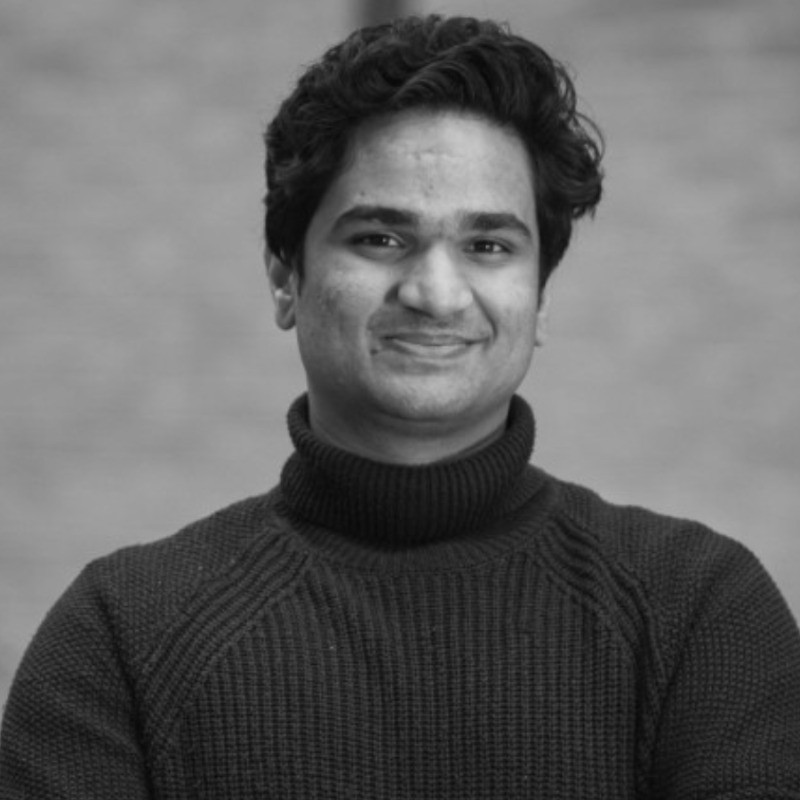
\includegraphics[width=2.0cm]{photo.jpg}
\end{minipage}
\vspace{-2pt}

% ================= SUMMARY =================
\section{Summary}
Applied Generative AI Engineer with 3 years of hands-on production experience architecting, shipping, and scaling production LLM applications, enterprise RAG pipelines, and autonomous agent workflows. Proven track record turning business use cases into scalable software solutions utilizing Python, SQL, modern vector databases, and multi-agent frameworks. Deep practical background implementing rigorous evaluation suites, context window optimization, and secure tool-calling patterns across European distributed platforms. Holder of an EU Long-Term Residence Permit (permanent unrestricted EU work authorization across all EU member states, no sponsorship required); based in Venice, Italy and available immediately for worldwide remote roles.

% ================= TECHNICAL EXPERTISE =================
\section{Technical Expertise}
\begin{itemize}
  \item \textbf{Generative AI \& Agent Frameworks:} LLM APIs (OpenAI, Anthropic), LangChain, agentic tool-use, multi-turn reasoning chains, structured JSON outputs, prompt tuning, human-in-the-loop approval gates.
  \item \textbf{RAG Pipelines \& Vector Search:} Retrieval-Augmented Generation, chunking strategies, hybrid search, dense embeddings, vector databases (pgvector, Chroma), metadata filtering, context reranking.
  \item \textbf{Software Development \& Backend Systems:} Python (FastAPI, asyncio, pandas, NumPy), SQL, TypeScript, Node.js, RESTful APIs, webhook orchestration, PostgreSQL schema modeling, Redis asynchronous task queues.
  \item \textbf{Cloud \& MLOps Practices:} Cloud environments (Azure, AWS), Docker containerization, CI/CD automation, automated regression and contract testing with Playwright, Git version control.
  \item \textbf{Languages \& Work Authorization:} English (C1 Professional, fluent), Hindi (Native), Italian (Beginner). EU Long-Term Residence Permit (unrestricted EU work authorization across all EU member states, no sponsorship required).
\end{itemize}

% ================= EXPERIENCE =================
\section{Experience}

\role{\href{https://flowspace.co}{FlowSpace.co}}{Mar 2024 - Aug 2026}{Lead Developer \& AI Systems Architect}{London, UK (remote)}
\begin{itemize}
  \item Architected and operated production customer-facing GenAI assistants and retrieval systems for a marketplace platform serving 4,500+ active enterprise users.
  \item Built resilient document parsing and ingestion pipelines with LLMs, translating unstructured partner data into validated JSON schemas and expanding live platform inventory.
  \item Designed multi-step agent reasoning chains with strict tool execution constraints and human-in-the-loop checkpoints, preventing ungrounded actions in customer-facing flows.
  \item Developed automated evaluation harnesses measuring grounding, precision, and latency against production transcripts, systematically lowering edge-case error rates.
  \item Maintained resilient TypeScript/Node.js microservices and PostgreSQL data models, utilizing asynchronous Redis queues to handle high-throughput query spikes.
  \item Implemented automated end-to-end regression test suites with Playwright, verifying API contracts and preventing system regressions across continuous release cycles.
\end{itemize}

\role{Urlink}{Apr 2025 - Jul 2025}{Project Manager \& Solutions Developer (Freelance)}{Barcelona, Spain (remote)}
\begin{itemize}
  \item Led technical discovery and implementation of customized web applications, data processing pipelines, and external API connectors for client platforms.
  \item Built automated data ingestion and transformation services connecting third-party partner APIs to PostgreSQL databases, maintaining strict data integrity and schema validation.
  \item Shipped interactive prototypes and API test harnesses to validate system boundaries and data flows prior to sprint execution, accelerating delivery timelines.
\end{itemize}

\role{Independent Technical Consultant}{Aug 2023 - Feb 2024}{AI Automation \& Integration Developer}{Venice, Italy}
\begin{itemize}
  \item Built and deployed custom LLM integrations, document retrieval prototypes, and webhook automation workflows for European enterprise clients using Python, TypeScript, and n8n.
  \item Replaced brittle manual document review workflows with automated LLM-assisted classification and extraction pipelines featuring comprehensive error handling and fallback routing.
  \item Authored technical architecture specifications, API documentation, and deployment guides to support client engineering teams in operating self-hosted workflows.
\end{itemize}

% ================= EDUCATION =================
\section{Education}
\role{Ca' Foscari University of Venice}{2020 - 2024}{BA in Philosophy, International Studies and Economics}{Venice, Italy}
\begin{itemize}
  \item Rigorous training in formal logic, analytical problem solving, systems analysis, and macroeconomic decision models.
\end{itemize}

\end{document}
